\documentclass[a4paper,14pt]{article}

\usepackage{comment} % Para comentar várias linhas ao mesmo tempo

%matemática
\usepackage{amsmath}
\usepackage{amssymb}

%diagramação
\usepackage{extsizes}
\everymath{\displaystyle}
\usepackage{geometry}
\usepackage{fancyhdr}
\usepackage{multicol}
\usepackage{graphicx}
\usepackage[brazil]{babel}
\usepackage[shortlabels]{enumitem}
\usepackage{cancel}
\usepackage{textcomp}
\usepackage{tcolorbox}

%tabelas
\usepackage{array} % Para melhor formatação de tabelas
\usepackage{longtable}
\usepackage{booktabs}  % Para linhas horizontais mais bonitas
\usepackage{float}   % Para usar o modificador [H]
\usepackage{caption} % Para usar legendas em tabelas
\usepackage{wrapfig} % Para usar tabelas e figuras flutuantes
\usepackage{xcolor} % Para cores do fundo de tabelas
\usepackage{colortbl} % Para cores do fundo de tabelas

%tikzpicture
\begin{comment}
	\usepackage{tikz}
	\usepackage{scalerel}
	\usepackage{pict2e}
	\usepackage{tkz-euclide}
	\usetikzlibrary{calc}
	\usetikzlibrary{patterns,arrows.meta}
	\usetikzlibrary{shadows}
	\usetikzlibrary{external}
\end{comment}


%pgfplots
\usepackage{pgfplots}
\pgfplotsset{compat=newest}
\usepgfplotslibrary{statistics}
\usepgfplotslibrary{fillbetween}

%colours
\usepackage{xcolor}



\columnsep=2cm
\hoffset=0cm
\textwidth=8cm
\setlength{\columnseprule}{.1pt}
\setlength{\columnsep}{2cm}
\renewcommand{\headrulewidth}{0pt}
\geometry{top=1in, bottom=1in, left=0.7in, right=0.5in}

\pagestyle{fancy}
\fancyhf{}
\fancyfoot[C]{\thepage}

\begin{document}
	
	\noindent\textbf{6FMA121, 6FMA122 - Matemática} 
	
	\begin{center}Probabilidade (Versão estudante)
	\end{center}
	
	\noindent\textbf{Nome:} \underline{\hspace{10cm}}
	\noindent\textbf{Data:} \underline{\hspace{4cm}}
	
	%\section*{Questões de Matemática}
	
	\begin{multicols}{2}
	    \noindent \begin{itemize}
	    	\item Dado um experimento cujo resultado não é totalmente previsível (experimento probabilístico), o espaço amostral é o conjunto de todos os resultados possíveis.
	    	\item Evento é qualquer subconjunto do espaço amostral que costuma representar algo que nos interessa.
	    	\item A probabilidade de um evento $E$, contido em um espaço amostral $S$, cujos elementos têm a mesma chance de ocorrer, é $\frac{n(E)}{n(S)}$.
	    \end{itemize}
		\noindent\textsubscript{--------------------------------------------------------------------------}
		\begin{enumerate} 
			\item Em um campeonato de natação, André, Bruno e Caio disputam a prova final. Quais são os possíveis resultados dessa competição? Qual é a probabilidade de André ficar em segundo lugar? \\\\\\\\\\\\\\\\\\\\\\\\\\
			\item Duas moedas são jogadas simultaneamente. Qual é a probabilidade de obtermos duas faces iguais? \\\\\\\\\\\\\\\\\\\\
			\item Júlio joga três moedas ao mesmo tempo. Qual é a probabilidade de ele:
			\begin{enumerate}[a)]
				\item obter exatamente duas caras. \\\\\\\\\\\\\\\\\\\\
				\item obter três coroas. \\\\\\\\
				\item obter pelo menos duas coroas? \\\\\\\\\\\\\\\\\\\\
			\end{enumerate}
			\item Ao jogar um dado honesto de seis faces, qual a probabilidade de obtermos:
			\begin{enumerate}[a)]
				\item um número ímpar de pontos? \\\\\\\\\\\\\\\\\\\\
				\item um número primo de pontos? \\\\\\\\\\\\\\\\\\\\\\\\
				\item 5 ou 6 pontos? \\\\\\\\\\\\\\\\\\\\
				\item 1 ponto? \\\\\\\\\\\\\\\\\\\\
			\end{enumerate}
			\item Num \textit{software}, foi feita uma simulação de lançamentos de dois dados. O espaço amostral desses lançamentos é: \\
			$S = \\ \{(1; 1), (1; 2), (1; 3), (1; 4), (1; 5), (1; 6), \\
			       (2; 1), (2; 2), (2; 3), (2; 4), (2; 5), (2; 6), \\
			       (3; 1), (3; 2), (3; 3), (3; 4), (3; 5), (3; 6), \\
			       (4; 1), (4; 2), (4; 3), (4; 4), (4; 5), (4; 6), \\
			       (5; 1), (5; 2), (5; 3), (5; 4), (5; 5), (5; 6), \\
			       (6; 1), (6; 2), (6; 3), (6; 4), (6; 5), (6; 6),
			     \}$
		    \begin{enumerate}[a)]
				\item Qual a probabilidade de obter 11 pontos? \\\\\\\\
				\item Qual é a probabilidade de o produto dos resultados dos dois dados ser múltiplo de 6? \\\\\\\\\\\\\\\\\\\\
				\item Os dados foram lançados e sabe-se que um deles deu 6. Qual é a probabilidade de que a soma dos resultados seja pelo menos 11? \\\\\\\\\\\\\\\\\\\\\\\\\\\\\\\\\\\\\\\\\\\\\\
		    \end{enumerate}
		    \textbf{Desafio olímpico} \\\\
		    (OBMEP) O gráfico de barras mostra a distribuição dos alunos de uma escola conforme o tempo diário dedicado à leitura. \\
		    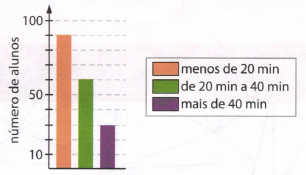
\includegraphics[width=1\linewidth]{6FMA121_imagens/imagem1}
		    Qual é o gráfico de setores que melhor representa, em amarelo, a fração de alunos que dedicam à leitura no máximo 40 minutos por dia? \\
		    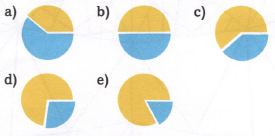
\includegraphics[width=1\linewidth]{6FMA121_imagens/imagem2} \newpage
		    %43 a 48
		    \item \begin{enumerate}[a)]
		    	\item Carlos lança três moedas. Quais são os possíveis resultados que ele irá encontrar? \\\\\\\\\\\\\\\\\\\\
		    	\item Se Carlos lançar um dado e uma moeda, qual será o espaço amostral? \\\\\\\\\\\\\\\\\\\\
		    \end{enumerate}
		    \item Durante uma gincana na escola de Maurício, 45 alunos deveriam ser divididos em dois times. Para facilitar, o professor distribuiu cartões numerados de 1 a 45. Os alunos que tiraram um número ímpar foram para o time vermelho. Sabe-se que Maurício tirou um número múltiplo de 3.
		    \begin{enumerate}[a)]
		    	\item Qual é a probabilidade de ele ter ficado no time amarelo? \\\\
		    	\item Qual é a probabilidade de ele ter ficado no time vermelho? \\\\\\\\\\\\\\\\\\\\
		    \end{enumerate}
		    \item Uma empresa de telefonia fabrica apenas dois modelos de celulares, Max e Mini, sempre lançados juntos. No mês de janelo foram fabricados 8 000 celulares. Se a probabilidade de a empresa fabricar um celular do modelo Max é de 0,35, quantos aparelhos do modelo Mini foram fabricados no mês de janeiro? \newpage
		    \item (Vunesp) Numa comunidade formada de 1 000 pessoas, foi feito um teste para detectar a presença de uma doença. Como o reste não é totalmente eficaz, existem pessoas doentes cujo resultado do teste foi negativo e existem pessoas saudáveis com resultado do teste positivo. Sabe-se que 200 pessoas da comunidade são portadoras dessa doença. Essa informação e alguns dos dados obtidos com o teste foram colocados na tabela seguinte.
		    Aqui está o código em LaTeX para criar a tabela solicitada, com as configurações especificadas:
	    	\begin{table}[H]
	    		\renewcommand{\arraystretch}{1.2} % Espaçamento entre as linhas
	    		\begin{tabular}{|m{2cm}|m{1.8cm}|m{2cm}|m{1.2cm}|}
	    			\hline
	    			\multicolumn{4}{|c|}{\textbf{Resultado do exame}} \\ \hline
	    			\textbf{Situação} & \textbf{Positivo ($P$)} & \textbf{Negativo ($N$)} & \textbf{Total} \\ \hline
	    			Saudável ($S$) & 80 & ~ & 800 \\ \hline
	    			Doente ($D$) & ~ & 40 & 200 \\ \hline
	    			Total & ~ & ~ & 1 000 \\ \hline
	    		\end{tabular}
	    	\end{table}
	    	\begin{enumerate}[a)]
	    		\item Complete a tabela com dados que estão faltando. \\\\\\\\\\\\\\\\\\\\\\
	    		\item Uma pessoa da comunidade é escolhida ao acaso e verifica-se que o resultado do teste foi positivo. Determine a probabilidade de essa pessoa ser saudável. \\\\\\\\\\\\\\\\\\\\
	    	\end{enumerate}
	    	\item Em uma escola, os alunos participaram de uma pesquisa sobre o destino de suas últimas férias. A tabela abaixo mostra o resultado dessa pesquisa:
	    	\begin{table}[H]
	    		\renewcommand{\arraystretch}{1.2} % Espaçamento entre as linhas
	    		\begin{tabular}{|m{4cm}|m{4cm}|}
	    			\hline
	    			\textbf{Local} & \textbf{Quantidade de alunos} \\ \hline
	    			Interior de SP & 320 \\ \hline
	    			Nordeste & 450 \\ \hline
	    			Norte & 180  \\ \hline
	    			Sul & 350 \\ \hline
	    			Centro-Oeste & 200 \\ \hline
	    			Exterior & 500 \\ \hline
	    			\textbf{Total} & \textbf{2 000} \\ \hline
	    		\end{tabular}
	    	\end{table}
	    	Escolhendo aleatoriamente um aluno que participou dessa pesquisa, responda: \newpage
	    	\begin{enumerate}[a)]
	    		\item qual é a probabilidade de esse aluno ter ido viajar para a região Norte do Brasil?
	    		\\\\\\\\
	    		\item qual é a probabilidade de esse aluno ter ido viajar para o interior de São Paulo?
	    		\\\\\\\\
	    	\end{enumerate}
	    	\item Uma turma de ex-alunos se reuniu para comemorar os 10 anos de formatura. Vários haviam se casado e tido filhos. Observe o gráfico abaixo com relação às 20 mulheres desse grupo.
	    	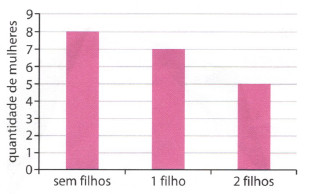
\includegraphics[width=1\linewidth]{6FMA121_imagens/imagem3}
	    	Escolhendo aleatoriamente uma das mulheres desse grupo, a probabilidade de ela ter um filho é:
	    	\begin{enumerate}[a)]
	    		\item 0,35
	    		\item 0,24
	    		\item 0,4
	    		\item 0,25
	    		\item 0,75
	    	\end{enumerate}
		\end{enumerate}
		$~$ \\ $~$ \\ $~$ \\ $~$ \\ $~$ \\ $~$ \\ $~$ \\ $~$ \\ $~$ \\ $~$ \\ $~$ \\ $~$ \\ $~$ \\ $~$ \\ $~$ \\ $~$ \\ $~$ \\ $~$ \\ $~$ \\ $~$ \\ $~$ \\ $~$ \\ $~$ \\ $~$ \\ $~$ \\ $~$ \\ $~$ \\ $~$ \\ $~$ \\ $~$ \\ $~$ \\ $~$ \\ $~$ \\ $~$ \\ $~$ \\ $~$ \\ $~$ \\ $~$ \\ $~$ \\ $~$ \\ $~$ \\ $~$ \\ $~$ \\ $~$
	\end{multicols}
\end{document}